\documentclass[tikz, border=10pt]{standalone}
\usepackage{amsmath, amssymb}
\usetikzlibrary{calc, positioning, arrows.meta, shapes.symbols, decorations.pathreplacing, backgrounds, fit, matrix}

\begin{document}
	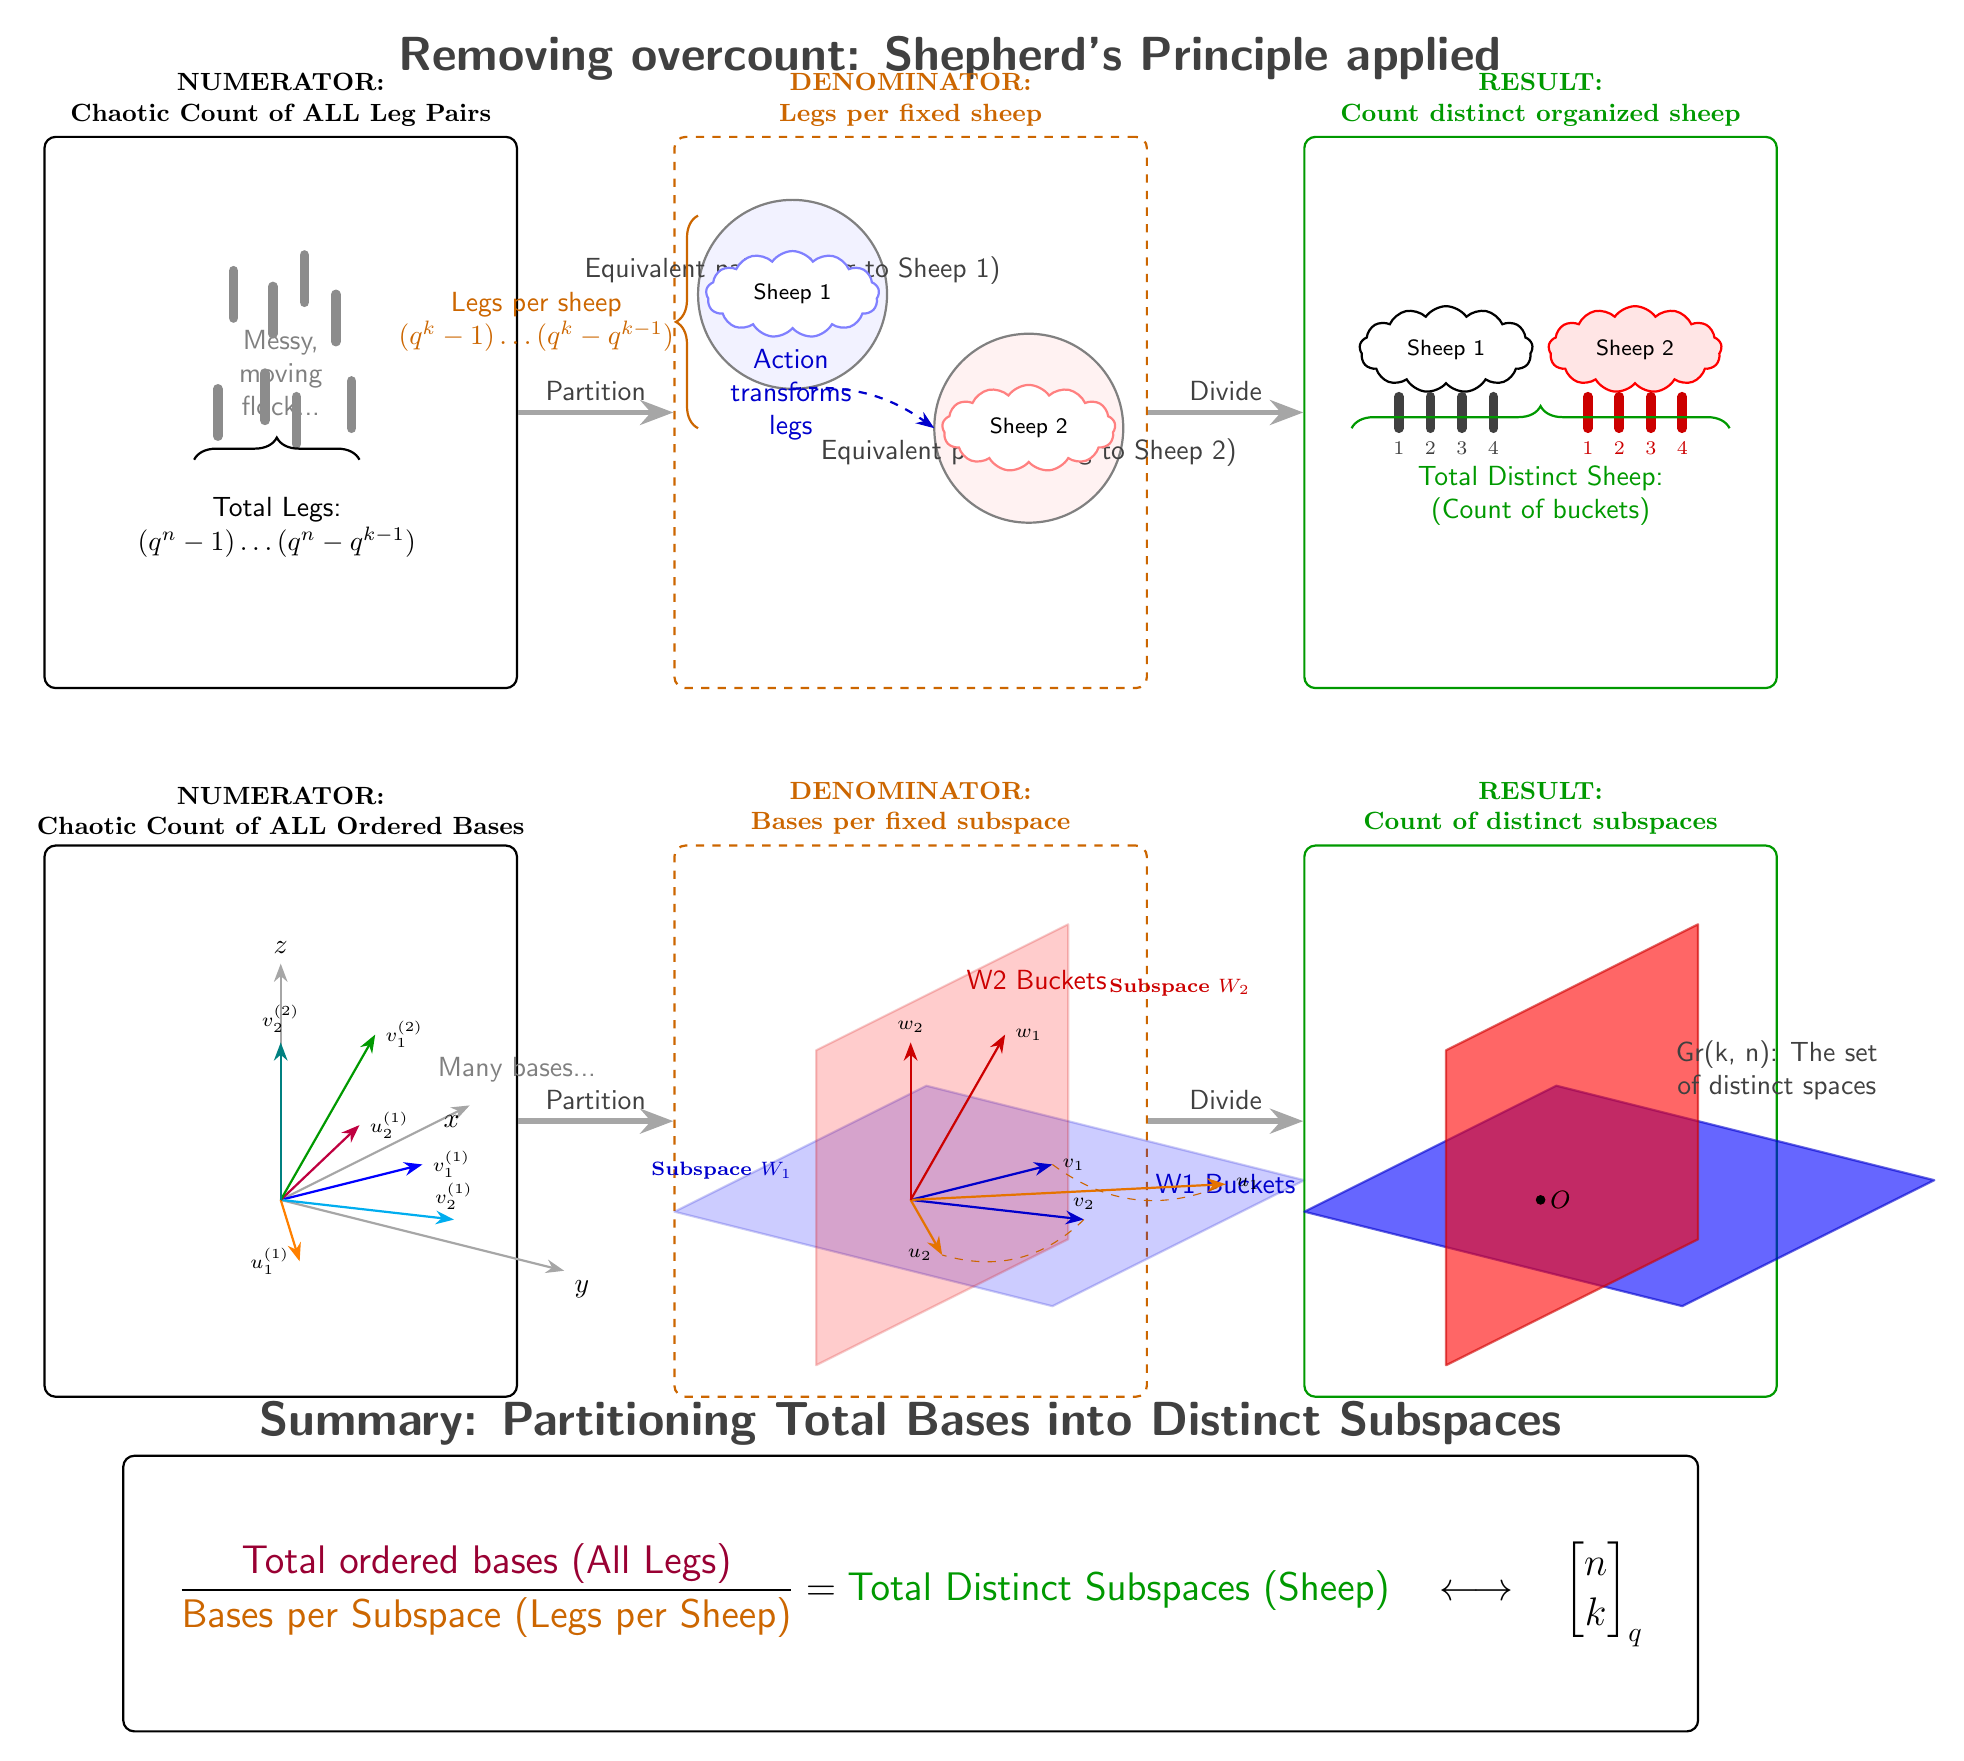
\begin{tikzpicture}[font=\sffamily,
		% Title & Text Styles
		mainTitle/.style={font=\sffamily\bfseries\LARGE, color=darkgray, align=center},
		term label/.style={font=\bfseries\small, align=center},
		% Arrow & Bracket Styles
		brace/.style={decorate, decoration={brace, amplitude=8pt}},
		Brace/.style={decorate, decoration={brace, amplitude=8pt, mirror}},
		mapArrow/.style={->, >=Stealth, dashed, thick},
		flowArrow/.style={->, >=Stealth, line width=2pt, color=gray!70},
		% 3D projection setup & styles
		perspective/.style={x={(0.8cm,0.4cm)}, y={(1.2cm,-0.3cm)}, z={(0cm,1cm)}},
		axis/.style={->, >=Stealth, draw=gray!70, thick},
		subspace/.style={opacity=.6, fill=#1, draw=#1!80!black, thick, line join=round},
		basis/.style={->, >=Stealth, thick}
		]
		
		% ==============================================================================
		% ROW 1: THE METAPHOR (SHEEP & LEGS) PARTITIONED
		% ==============================================================================
		\node[mainTitle] at (4.5, 9.5) {Removing overcount: Shepherd's Principle applied};
		
		% --- LEFT PANEL: OVERCOUNT (Total Legs) ---
		\node[draw, thick, rounded corners, minimum width=6cm, minimum height=7cm, label={[term label]above:NUMERATOR:\\Chaotic Count of ALL Leg Pairs}] (MetaphorNum) at (-4, 5) {};
		\node[align=center, text=gray] at (-4, 5.5) {Messy,\\ moving\\ flock...};
		
		\begin{scope}[shift={(0,5)}]
			% Cluster of scattered legs
			\foreach \x/\y in {-4.6/1.2, -4.1/1.0, -3.7/1.4, -3.3/0.9,
				-4.8/-0.3, -4.2/-0.1, -3.8/-0.4, -3.1/-0.2} {
				\draw[line width=3.5pt, color=darkgray!60, line cap=round] (\x, \y) -- (\x, \y+0.6);
			}
			\draw[Brace, thick] (-3.0, -0.6) -- (-5.1, -0.6) node[midway, below=10pt, align=center] {Total Legs:\\$(q^n-1)\dots(q^n-q^{k-1})$};
		\end{scope}
		
		% --- MIDDLE PANEL: GROUPING (Buckets/ Sheep) ---
		\node[draw, thick, dashed, orange!80!black, rounded corners, minimum width=6cm, minimum height=7cm, label={[term label, text=orange!80!black]above:DENOMINATOR:\\Legs per fixed sheep}] (MetaphorDen) at (4, 5) {};
		
		\begin{scope}[shift={(4,5)}]
			% Two buckets/ equivalence classes
			\draw[thick, gray, fill=blue!5] (-1.5, 1.5) circle (1.2cm) node[above, text=darkgray] {Equivalent pairs\\(belong to Sheep 1)};
			\node[cloud, cloud puffs=13, cloud puff arc=110, aspect=2.2, draw=blue!50, thick, fill=white, minimum width=2.2cm, minimum height=1.1cm] at (-1.5, 1.5) {\footnotesize Sheep 1};
			
			\draw[thick, gray, fill=red!5] (1.5, -0.2) circle (1.2cm) node[below, text=darkgray] {Equivalent pairs\\(belong to Sheep 2)};
			\node[cloud, cloud puffs=13, cloud puff arc=110, aspect=2.2, draw=red!50, thick, fill=white, minimum width=2.2cm, minimum height=1.1cm] at (1.5, -0.2) {\footnotesize Sheep 2};
			
			% The reduction factor (Bases per space)
			\draw[mapArrow, blue!80!black] (-1.5, 0.3) to[bend left=20] node[midway, left=2pt, align=center] {Action\\transforms\\legs} (0.3, -0.2);
			\draw[Brace, orange!80!black, thick] (-2.7, 2.5) -- (-2.7, -0.2) node[midway, left=5pt, align=center] {Legs per sheep\\$(q^k-1)\dots(q^k-q^{k-1})$};
		\end{scope}
		
		% --- RIGHT PANEL: DISTINCT RESULT (Buckets Counted) ---
		\node[draw, thick, green!60!black, rounded corners, minimum width=6cm, minimum height=7cm, label={[term label, text=green!60!black]above:RESULT:\\Count distinct organized sheep}] (MetaphorRes) at (12, 5) {};
		
		\begin{scope}[shift={(12,5)}]
			% Two distinct, organized sheep
			\begin{scope}[shift={(-1.2, 0)}]
				\node[cloud, cloud puffs=13, cloud puff arc=110, aspect=2.2, draw=black, thick, fill=white, minimum width=2.2cm, minimum height=1.1cm] at (0, 0.8) {\footnotesize Sheep 1};
				\draw[line width=3.5pt, color=darkgray, line cap=round] (-0.6, 0.2) -- (-0.6, -0.2) node[below, font=\scriptsize] {1};
				\draw[line width=3.5pt, color=darkgray, line cap=round] (-0.2, 0.2) -- (-0.2, -0.2) node[below, font=\scriptsize] {2};
				\draw[line width=3.5pt, color=darkgray, line cap=round] (0.2, 0.2) -- (0.2, -0.2) node[below, font=\scriptsize] {3};
				\draw[line width=3.5pt, color=darkgray, line cap=round] (0.6, 0.2) -- (0.6, -0.2) node[below, font=\scriptsize] {4};
			\end{scope}
			
			\begin{scope}[shift={(1.2, 0)}]
				\node[cloud, cloud puffs=13, cloud puff arc=110, aspect=2.2, draw=red, thick, fill=red!10, minimum width=2.2cm, minimum height=1.1cm] at (0, 0.8) {\footnotesize Sheep 2};
				\draw[line width=3.5pt, color=red!80!black, line cap=round] (-0.6, 0.2) -- (-0.6, -0.2) node[below, font=\scriptsize] {1};
				\draw[line width=3.5pt, color=red!80!black, line cap=round] (-0.2, 0.2) -- (-0.2, -0.2) node[below, font=\scriptsize] {2};
				\draw[line width=3.5pt, color=red!80!black, line cap=round] (0.2, 0.2) -- (0.2, -0.2) node[below, font=\scriptsize] {3};
				\draw[line width=3.5pt, color=red!80!black, line cap=round] (0.6, 0.2) -- (0.6, -0.2) node[below, font=\scriptsize] {4};
			\end{scope}
			
			\draw[Brace, green!60!black, thick] (2.4, -0.2) -- (-2.4, -0.2) node[midway, below=10pt, align=center] {Total Distinct Sheep:\\(Count of buckets)};
		\end{scope}
		
		% --- CONNECTING FLOW ---
		\draw[flowArrow] (MetaphorNum.east) -- (MetaphorDen.west) node[midway, above, text=darkgray] {Partition};
		\draw[flowArrow] (MetaphorDen.east) -- (MetaphorRes.west) node[midway, above, text=darkgray] {Divide};
		
		
		% ==============================================================================
		% ROW 2: THE MATHEMATICS PARTITIONED (2D in 3D perspective)
		% ==============================================================================
		\begin{scope}[shift={(0, -4)}, scale=1]
			
			% --- LEFT PANEL: OVERCOUNT (Total Bases) ---
			\node[draw, thick, rounded corners, minimum width=6cm, minimum height=7cm, label={[term label]above:NUMERATOR:\\Chaotic Count of ALL Ordered Bases}] (MathNum) at (-4, 0) {};
			\begin{scope}[shift={(-4, -1)}, perspective]
				% Ambient 3D axes
				\draw[axis] (0,0,0) -- (3,0,0) node[anchor=north east]{$x$};
				\draw[axis] (0,0,0) -- (0,3,0) node[anchor=north west]{$y$};
				\draw[axis] (0,0,0) -- (0,0,3) node[anchor=south]{$z$};
				
				% Plot many individual vector tuples
				\draw[basis, draw=blue] (0,0,0) -- (1.5, 0.5, 0) node[right, font=\scriptsize] {$v_1^{(1)}$};
				\draw[basis, draw=cyan] (0,0,0) -- (0.5, 1.5, 0) node[above, font=\scriptsize] {$v_2^{(1)}$};
				\draw[basis, draw=orange] (0,0,0) -- (-1.2, 1.0, 0) node[left, font=\scriptsize] {$u_1^{(1)}$};
				\draw[basis, draw=purple] (0,0,0) -- (2.0, -0.5, 0) node[right, font=\scriptsize] {$u_2^{(1)}$};
				
				\draw[basis, draw=green!60!black] (0,0,0) -- (1.5, 0, 1.5) node[right, font=\scriptsize] {$v_1^{(2)}$};
				\draw[basis, draw=teal] (0,0,0) -- (0, 0, 2) node[above, font=\scriptsize] {$v_2^{(2)}$};
				
				\node[align=center, text=gray] at (1.5, 1.5, 1.5) {Many bases...};
			\end{scope}
			
			% --- MIDDLE PANEL: GROUPING (Buckets/ Distinct Subspaces explained) ---
			\node[draw, thick, dashed, orange!80!black, rounded corners, minimum width=6cm, minimum height=7cm, label={[term label, text=orange!80!black]above:DENOMINATOR:\\Bases per fixed subspace}] (MathDen) at (4, 0) {};
			\begin{scope}[shift={(4, -1)}, perspective]
				
				% Partitioning logic: group bases that span the same subspace
				\draw[subspace=blue, opacity=.2] (2.5,2.5,0) -- (-1.5,2.5,0) -- (-1.5,-1.5,0) -- (2.5,-1.5,0) -- cycle;
				\node[text=blue!80!black] at (2,2,0) {W1 Buckets};
				
				\draw[subspace=red, opacity=.2] (2.5,0,2.5) -- (-1.5,0,2.5) -- (-1.5,0,-1.5) -- (2.5,0,-1.5) -- cycle;
				\node[text=red!80!black] at (2,0,2) {W2 Buckets};
				
				% For subspace W1 (blue plane), explicitly show overcounting
				\draw[basis, draw=blue!80!black] (0,0,0) -- (1.5, 0.5, 0) node[right, font=\scriptsize] {$v_1$};
				\draw[basis, draw=blue!80!black] (0,0,0) -- (0.5, 1.5, 0) node[above, font=\scriptsize] {$v_2$};
				\draw[basis, draw=orange!90!black] (0,0,0) -- (2.0, 2.0, 0) node[right, font=\scriptsize] {$u_1$};
				\draw[basis, draw=orange!90!black] (0,0,0) -- (-1.0, 1.0, 0) node[left, font=\scriptsize] {$u_2$};
				
				\node[below, text=blue!80!black, font=\scriptsize\bfseries] at (0,-2,0) {Subspace $W_1$};
				
				% Dashed equivalence connections
				\draw[dashed, orange!80!black] (1.5, 0.5, 0) to[bend right] (2.0, 2.0, 0);
				\draw[dashed, orange!80!black] (0.5, 1.5, 0) to[bend left] (-1.0, 1.0, 0);
				
				% For subspace W2 (red plane)
				\draw[basis, draw=red!80!black] (0,0,0) -- (1.5, 0, 1.5) node[right, font=\scriptsize] {$w_1$};
				\draw[basis, draw=red!80!black] (0,0,0) -- (0, 0, 2) node[above, font=\scriptsize] {$w_2$};
				\node[right, text=red!80!black, font=\scriptsize\bfseries] at (3,0,1.5) {Subspace $W_2$};
				
			\end{scope}
			
			% --- RIGHT PANEL: DISTINCT RESULT (Grassmannian visualized) ---
			\node[draw, thick, green!60!black, rounded corners, minimum width=6cm, minimum height=7cm, label={[term label, text=green!60!black]above:RESULT:\\Count of distinct subspaces}] (MathRes) at (12, 0) {};
			\begin{scope}[shift={(12, -1)}, perspective]
				% Just the distinct, tilted planes are counted. Bases are removed.
				\filldraw[subspace=blue] (2.5,2.5,0) -- (-1.5,2.5,0) -- (-1.5,-1.5,0) -- (2.5,-1.5,0) -- cycle;
				\filldraw[black] (0,0,0) circle (1.5pt) node[right, font=\small\bfseries] {$O$};
				
				\filldraw[subspace=red] (2.5,0,2.5) -- (-1.5,0,2.5) -- (-1.5,0,-1.5) -- (2.5,0,-1.5) -- cycle;
				\filldraw[black] (0,0,0) circle (1.5pt) node[right, font=\small\bfseries] {$O$};
				
				\node[align=center, text=darkgray] at (1.5, 1.5, 1.5) {Gr(k, n): The set\\ of distinct spaces};
			\end{scope}
			
			% --- CONNECTING FLOW ---
			\draw[flowArrow] (MathNum.east) -- (MathDen.west) node[midway, above, text=darkgray] {Partition};
			\draw[flowArrow] (MathDen.east) -- (MathRes.west) node[midway, above, text=darkgray] {Divide};
		\end{scope}
		
		% ==============================================================================
		% ROW 3: SUMMARY FRACTION & LEGEND
		% ==============================================================================
		\node[draw, thick, rounded corners, minimum width=20cm, minimum height=3.5cm, fill=white, label={[mainTitle]above:Summary: Partitioning Total Bases into Distinct Subspaces}] (FinalSummary) at (4, -10) {
			\Large $\displaystyle \frac{\text{\textcolor{purple!80!black}{Total ordered bases (All Legs)}}}{\text{\textcolor{orange!80!black}{Bases per Subspace (Legs per Sheep)}}} = \mathbf{\text{\textcolor{green!60!black}{Total Distinct Subspaces (Sheep)}}} \quad \longleftrightarrow \quad \begin{bmatrix} n \\ k \end{bmatrix}_q$
		};
		
	\end{tikzpicture}
\end{document}